\documentclass{article}
\usepackage[utf8]{inputenc}
\usepackage[nottoc]{tocbibind}
\usepackage{natbib}
\usepackage{url}
\usepackage{amssymb}
\usepackage[superscript,biblabel]{cite}

\usepackage{pgfplots}
\usepackage{pgfplotstable}
\usepackage{booktabs}
\usepackage{array}
\usepackage{colortbl}

\setcounter{section}{-1}

\pgfplotstableset{% global configuration
  every head row/.style={before row=\toprule,after row=\midrule},
  every last row/.style={after row=\bottomrule},
  fixed,precision=4,
}

\makeatletter
\setlength{\@fptop}{0pt}
\setlength{\@fpbot}{0pt plus 1fil}
\makeatother

\begin{document}
\begin{titlepage}
    \begin{center}
        \vspace*{1cm}
        
        \Large
        \textbf{An Investigation into the use of Genetic Algorithms to design and optimise Screening Rules to be used in automatic stock trading}
        
        \vspace{0.5cm}
        \large
        Presented for the degree of \\
        Master in Science for Mathematics and Computer Science
        
        \vspace{0.5cm}
        \textbf{Dominic Walters}
        \vfill
        
        
\includegraphics[width=0.4\textwidth]{images/uobLogo.png}
        
        \vspace{0.5cm}
        Supervisor: Shan He\\
        \vspace{0.5cm}
        School of Computer Science\\
        University of Birmingham\\
        England, United Kingdom\\
        08/04/2019
    \end{center}
\end{titlepage}
\tableofcontents
\section{Abstract}


All software for this project can be found at: \newline \url{https://git-teaching.cs.bham.ac.uk/mod-ug-proj-2018/dxw407}.
\section{Introduction}
\subsection{The Stock Market}
The stock market is ubiquitous within modern life. Any time you look at the news, it will be featured. References to stock indices such as the NASDAQ Composite, FTSE 100, Dow Jones, or the S\&P 500 permeate any discussion of the western economy in the modern day, and yet very few people actually interact directly with the market. \newline

The average person does not buy stocks, the closest they get is investing in an ISA through their bank (and not even all ISAs invest in stocks). The prevailing reason for this is that, as a casual investor, it is simply too difficult to participate in stock trading and make a reasonable return. The average person does not understand the majority of the statistics behind stock trading, and they don't understand the basics of when to buy and when to sell. \newline

This is where stock screeners come in; they provide a simple way to filter out stocks that are wholly inappropriate to invest in. However, a large amount of currently widely used screening strategies are years (if not decades) old, raising doubts as to their efficacy. Could the generation of newer, more up to date screening rules be automated? And if so, would these automatically generated rules perform to a competitive standard in the modern market?

\subsection{Generating Screening Rules}
I suggest an investigation into the efficacy of creating an algorithm that generates profitable stock screening rules, by utilising evolutionary machine learning techniques. This algorithm would run over as much historical data as possible, and provide new screening strategies that are as up to date as the data it uses. \newline

Such an algorithm would allow traders (both casual and professional) to remain up to date with current market trends, as the screening rules would adapt to changes in the economy over time. If a strategy begins to perform poorly, a new one can be automatically generated to replace it. \newline

Generating valid screening strategies would be the logical first step, but once generated how can a value be assigned to these strategies?

\subsection{Measuring Effectiveness}
\subsubsection{Playing the Stock Market Game}
A screening rule is only as good as the return that it obtains on the stocks that it purchases. As such, the most natural way to evaluate a screening rule is to see what yearly return it gets on the stocks that it suggests should be purchased. There are a variety of choices to be made here:
\begin{itemize}
    \item When should the strategy choose to sell the stocks that it purchases?
    \vspace{-2mm}
    \item What should be done if a prospective stock does not provide a field that the strategy requires?
    \vspace{-2mm}
    \item What time period should the rule be evaluated over?
    \vspace{-2mm}
    \item What data should be used in this evaluation?
\end{itemize}

Once these choices are made and a value is assigned to each strategy, how can these values be contextualised with regards to actual stock trading returns in the real world? What does it mean to achieve a ``good'' return?

\subsubsection{Market Indices} \label{snpPls}
One of the simplest and most risk-free ways to invest your money in the real world is to buy an index fund. An index fund is a stock portfolio that is constructed to track a prominent market index. Such market indices include the aforementioned NASDAQ Composite, Dow Jones, and S\&P 500 from the American market, and the variety of FTSE indices from the UK market. \newline

A market index is a portfolio of stocks that are used to measure some specific section of the market. For example, the three most often used American indices: 

\begin{itemize}
    \item \bf Dow Jones \rm - The Dow represents the value of 30 large, publicly owned businesses within the United States. These businesses are chosen by a committee. The index value is the amount of money required, in dollars, to purchase one stock from each of the 30 companies.
    \item \bf NASDAQ Composite \rm - The NASDAQ Composite represents a market-capitalisation-weighted value of all of the companies traded on the NASDAQ stock exchange, of which there are approximately 3,300.
    \item \bf S\&P 500 \rm - The S\&P 500 represents the market-capitalisation-weighted value of 500 specific American companies. These companies are selected by a committee based on a set of 8 criteria including:  market capitalization, financial viability, and the length of time that they have been publicly traded.
\end{itemize}

Of these three, the S\&P 500 is widely considered to be the best representation of the US Stock Market. \cite{snp500Best} Warren Buffett, one of the world's leading investors and perhaps the most famous person involved with the US stock market, has said that he has a ``tough time'' trying to outdo the returns of the S\&P 500 Index. Furthermore, he has said that personally he would ``buy the S\&P in a second''. \cite{buffettsnp} \newline

Therefore, to contextualise the screening rules that my algorithm will create, I will evaluate their yearly return against the yearly return of the S\&P 500 index. \newline


\section{Project Layout}
The project can be split into 3 core sections.

\subsection{The Simulation Game} \label{simGameProp}
In order to train a genetic algorithm over historical data, we have to create some form of “payoff” for each of the proposed screening strategies in the population, that is representative of how much profit that strategy would create when choosing stocks to buy/sell in the real economy. \newline

My proposed way to achieve this is to play a simulated stock trading “game”. For each prospective screening rule, run through as many quarters of historical data as possible. For each quarter, the screening strategy buys all stocks that satisfy it from the quarter. At the end of the game, the net worth of the strategy is calculated and a payoff is assigned based on the profit attained. \newline

This payoff is then used to perform the selection function required for the genetic algorithm, as well as to contextualise the created screening strategies and compare to the returns of the S\&P 500.

\subsection{The Evolutionary Algorithm} \label{evoAlgoProp}
The pseudo-code for a generic evolutionary algorithm is as follows:
\begin{enumerate}
    \item \bf Initialisation \rm - Generate initial population $gen_{0}$ \vspace{-2mm}
    \item For g from \{1, 2, .., G\}
    \begin{enumerate}
        \item Create blank population $gen_{g}$
        \item For \_n from \{0, 1, .., size of $gen_{g-1}$ - 1\}
        \begin{enumerate}
            \item \bf Selection \rm - Select two members of $gen_{g-1}$, biasing to members with higher \bf Fitness Function \rm values
            \item \bf Crossover \rm - Create a new member by crossover of the two selected members
            \item \bf Mutation \rm - Mutate the new member
            \item Add the new member to $gen_{g}$
        \end{enumerate}
    \end{enumerate} \vspace{-2mm}
    \item Return $gen_{G}$
\end{enumerate}

I intend to begin with this generic framework, and then adapt my algorithm as needed. However, not all of this standard version is straight forward and easy to implement within the search space I am considering. Specifically:
\begin{itemize}
    \item \bf Generation of Initial Population \rm 
    \item \bf Computation of the Fitness Function \rm
    \item \bf The Crossover Function \rm
\end{itemize}

This section of the system will require experimentation, as the initialisation and crossover methods will need to be specially designed for this search space. The crossover function is going to be the hardest element to construct. \newline

It has to allow a combination of two screening rules of a hundred variables each (at a minimum), all representing different aspects of a stock (with different scales and potentially wildly different values), in such a way that the result will on average be a better screening strategy. This won't be a trivial function to design.

\subsection{Testing and Experimentation}
Once the algorithm is established and providing valid results, a series of evaluations should be run to determine the quality of the screening strategies provided. This is likely to be a highly iterative process: a test is run, an improvement suggested, the test is rerun with the improvement. \newline

Additionally, more complicated evolutionary methods could be tested: niching and speciation strategies, elitism, co-evolution, and multi-objective optimisation to name a few. It is also at this stage that the algorithm’s variables can be tuned to attain the best screening rule possible. \newline

Evaluation of the system is very open-ended in nature, only really limited by what can be achieved before the deadline.
\section{Literature Review}
\subsection{Preamble}
There is a rich variety of research available in the field of applying machine learning techniques to stock market trading. The earliest originate in the late 90's and cover a range of very specific niches within the field, from portfolio management and stock price forecasting, to establishing trading rules for automatic stock screeners. \newline

To achieve these aims, an assortment of different machine learning techniques are utilised. Notably, the style of machine learning changes over time, with Genetic Algorithms being more popular in the early 00's and Neural Networks being the current go-to method.

\subsection{Financial Forecasting Using GAs \cite{mahfoudMani}}
This first paper outlines ``a new system that utilizes genetic algorithms...to predict the future performances of individual stocks''.

\subsubsection{Genetic Algorithms and Chromosomes}

It begins by outlining the basic terminology within Machine Learning and Genetic Algorithms, particularly the concepts of Mutation and Crossover within the field of GAs. A key term defined early on is ``genetic material'' (nowadays commonly referred to as the Chromosome or the Genotype). The Chromosome (Genotype) is a set of parameters which define a proposed solution (Phenotype). In layman's terms, the solution is a specific realisation of the chromosome. \newline

The author makes a key distinction here, saying that the algorithm ``implicitly processes...the genetic material (chromosomes)...and not individual solutions''. This is an important separation of concepts; the algorithm does not transform existing solutions into new solutions, it transforms the set of possible solutions into a new set of possible solutions, which is ``better'' in some definable fashion. \newline

The paper then gives a specific example saying ``...a GA may discover that one variable, such as price-to-earnings ratio, is a better indicator of future return than another, such as past return''. This is the core feature of genetic algorithms that enable them to search their domain more efficiently; they can bias in favour of the better ``dimension'', the more important rule in the chromosome.

\subsubsection{Michigan Vs Pittsburgh}

There are two approaches to how populations work within genetic algorithms. Either the population in its entirety forms one chromosome with each member being one part of that chromosome (Michigan approach), or every member is a chromosome and the population is a pool of viable chromosomes (Pittsburgh approach). This study in particular uses the Michigan approach, whilst I intend to use Pittsburgh. \newline

The reason given in the study for this choice is that Pittsburgh constitutes a ``large handicap on a GA-based learner'', in terms of time efficiency. However, this is a paper from 20 years ago and concerns of learning speed due to large data size are far less relevant in the modern day. The vast majority of modern genetic algorithms use the Pittsburgh approach, as it is conceptually closer to the idea of evolution that the algorithm endeavours to recreate.

\subsubsection{Niching}

A short discussion on the benefits of niching comes next. Niching is the process of only allowing chromosomes to compete with each other if they are sufficiently similar. This can allow a good deal of variation to be present within the population, as the algorithm can optimise multiple potential chromosomes at once, each chromosome being wildly different. \newline

The author goes on to specify that this is a useful construct within the field of financial prediction as ``different rules within a single population can perform forecasting under different market environments''.

\subsubsection{The Experiments}

The core of the study consists of two experiments, both effectively the same but the second at a larger scale; presumably this was done in case the second experiment wasn't successful so the authors would at least have something to report. Due to the similarity between these experiments, I am going to ignore the first one. \newline

In both experiments the authors genetic algorithm is compared to a neural network performing the same task. The task here is the classification of stocks into three categories: buy, sell, and no opinion. The algorithm is set up such that ``both GA and NN forecasts are made at the end of the week for three consecutive weeks. Each weekend, forecasts are made for over 1600 stocks. Twelve weeks after each forecast, the forecasts are compared with actual 12-week relative returns.'' \newline

The GA and NN predict both the ``magnitude and direction of the return of each stock, relative to the market''. Extra statistics are then calculated such as the average returns of the positive and negative forecasts, as well as a measure of the spread between these two averages, with high spread implying a better set of predictions.

\subsubsection{The Results}

The GAs outperformed the NNs overall with a larger spread (2.16\% versus 1.4\%) and better mean relative return performance over the top two quintiles (typically only stocks in the top two quintiles of this statistic are traded). \newline

The author goes on to reference a prior paper by Mahfoud \& Mani from 1995, suggesting that ``an approach that utilizes both GA and NN forecasts is superior to utilizing the better of the two algorithms, in isolation''. The author demonstrates that this hypothesis was correct in this experiment, with ``an average relative return of 6.61\% in the top quintile of the positive combined forecasts. This is a 21\% improvement over the GAs alone, and a 50\% improvement over the NNs alone.''

\subsubsection{GA versus NN}

The final discussion the author presents is whether GAs or NNs are better for this style of application. The author does not conclude that either method is superior to the other, referring to both methods as ``promising''. The author continues, suggesting that this promise is ``due to their ability to learn nonlinear relationships ... (that) are typically not apparent to the average market participant''. In other words, the algorithms can spot trends that a human observer (or a less sophisticated computer method) could not reliably notice. \newline

The author attributes the better performance of the GAs to their ability to abstain from predicting (which was done 27\% of the time), whereas the neural network was forced to always predict. This is quite a significant functional difference, which throws the overall result into doubt; the comparison between the two systems is hardly fair if only one of them enjoys more advanced features. \newline

The last comment that I wish to highlight is that GAs have the ability to output ``comprehensible rules''. Unlike black box methods like NNs, the GAs output can be easily designed to be human readable. This allows the output of the GA to be easily examined, and for it to be compared - immediately and directly - with human designed methods.

\subsection{Using GAs to find Technical Trading rules \cite{allenKarjalainen}}
This second study experiments with a genetic algorithm ``to learn technical trading rules for the S\&P 500 index using daily prices from 1928 to 1995.'' This is much closer to what I am trying to achieve than the first paper.

\subsubsection{Introduction}
The paper begins by stating its purpose: ``to demonstrate how they (Genetic Algorithms) can be used to find technical trading rules.'' It continues with a presentation of past literature, stating that ``such rules do not make money''. \newline

A number of studies are referenced, including Fama (1970) which ``dismiss(ed) technical analysis as a futile undertaking'' \cite{fama70}. Brock et al. (1992) was slightly more hopeful, showing that ``in the absence of transaction costs ... these rules identify periods to be in the market when returns are high and volatility is low (and vice versa)'' \cite{brock92}.

\subsubsection{Genetic Algorithms Overview}
The second chapter presents an overview of the basics of Evolutionary Algorithms as well as Genetic Programming. I am motivated to skip this section as I intend to provide my own summary of the relevant concepts within Evolutionary Algorithms in a later chapter, but also, there are several statements from this chapter which are no longer accurate. \newline

For example, the author states that ``solution candidates are represented as character strings from a given (often binary) alphabet.'' Whilst this is still a valid method to represent solution candidates, advances in the complexity of computers have allowed for more elaborate representations than simple bit strings. \newline

There is a related comment later in the section stating that evolutionary algorithms ``embody very little problem-specific knowledge''. This is incorrect; evolutionary algorithms can be customised in a variety of ways to their problem domain, most specifically with regards to the fitness function (which the author themselves concedes in chapter 2.1 paragraph 2) and problem representation. A custom representation then demands at least custom crossover and mutation functions, and perhaps even requiring a custom selection function as well.

\subsubsection{Representing Trading Rules}
After introducing Genetic Programming in the last chapter, the authors go into detail as to how they will represent their trading rules as genetic programs. \newline

The rules are constructed as trees, from a variety of mathematical and logical operators. Each tree corresponds to a boolean expression which at any point in time is either true or false. The authors provide two simple example rules:
\begin{figure}[h]
    \centering
    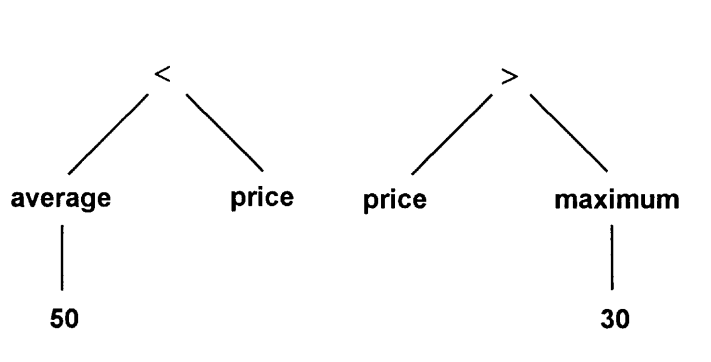
\includegraphics[width=0.5\textwidth]{images/averageAndMax.png}
\end{figure}

The left tree represents a rule which evaluates true if the current stock price is greater than a 50 day moving average of the stock price, and the right represents a rule which evaluates true if the current stock price is greater than the 30 day maximum stock price. \newline 

The author continues by defining the necessary crossover operator for this tree representation, as well as an appropriate fitness function.

\subsubsection{Overfitting}
After discussing representation, the author stresses the need to address the ``possibility of overfitting the training data''. Overfitting can occur in machine learning algorithms for a variety of reasons, but most stem from having a lack of data:
\begin{itemize}
    \item Small Data Set - The algorithm can only detect trends over the data it has. If the data set is small, the algorithm has less chance to detect common trends.
    \item Training Data Reuse - Small data sets may necessitate that the algorithm be repeatedly trained over the same data. Unless precautions are taken, this may result in the algorithm learning the data set as opposed to learning its trends.
    \item Evaluating on Training Data - If the algorithm is evaluated on data that it has already seen (data that it was trained on), then it is likely to give inaccurate results.
\end{itemize}

The author proposes a series of options to tackle this overfitting, including ``reserving
a part of the data as a validation set on which to test the predictions, increasing
the amount of training data, penalizing for model complexity, and minimizing
the amount of information needed to describe both the model and the data''. The author opts to implement the first of these suggestions.

\subsubsection{Results}
The results of the algorithm are not particularly encouraging. Running their algorithm 100 times, the authors generate 89 trading rules. The excess return of these rules is predominantly negative (meaning that the rules did not outperform the strategy of buying and holding), and the trading frequency is low with 3.8 trades per year on average. The results are marginally better when transaction fees are lowered, and marginally worse when they are increased. \newline

The author summarises, saying ``the out-of-sample test results indicate that the trading rules do not earn consistent excess returns after transaction costs. Nevertheless, they appear to have some ability to forecast daily returns.'' \newline

They end with some criticisms on their algorithm, specifically that their ``parameters are not necessarily optimal'', as well as stating that ``it would be interesting to apply a similar technique to learn fundamental trading rules,'' which is what I intend to do with my algorithm.
\section{Prerequisite Knowledge}
Before I discuss the implementation of my proposal I will define some terminology which I can draw from in later sections.
\subsection{Genetic Algorithms}
The concept of a Genetic Algorithm (also called an Evolutionary Algorithm) originates - as much of modern Computer Science does - with Alan Turing \cite{turingImitation}. He proposed a schema for a ``learning machine'' which borrowed from the ideas of Darwinian Natural Selection, to learn by a process that would be ``more expeditious than evolution''.

\subsubsection{Structure} \label{Structure}
Classical Genetic Algorithms share a common structure shown earlier in \ref{evoAlgoProp}:
\begin{enumerate}
    \item \bf Initialisation (\ref{Initialisation}) \rm - Generate initial population $gen_{0}$
    \item For g from \{1, 2, .., G\}
    \begin{enumerate}
        \item Create blank population $gen_{g}$
        \item For \_n from \{0, 1, .., size of $gen_{g-1}$ - 1\}
        \begin{enumerate}
            \item \bf Selection (\ref{Selection}) \rm - Select two members of $gen_{g-1}$, biasing to members with higher \bf Fitness Function (\ref{Fitness}) \rm values
            \item \bf Crossover (\ref{Crossover}) \rm - Create a new member by crossover of the two selected members
            \item \bf Mutation (\ref{Mutation}) \rm - Mutate the new member
            \item Add the new member to $gen_{g}$
        \end{enumerate}
    \end{enumerate}
    \item Return $gen_{G}$
\end{enumerate}

This structure is intentionally vague as each stage of the algorithm can be designed and tailored to the form of the search space on which it is searching. \newline

For example, a GA that is searching some 3D surface in an optimisation problem for the highest point could use a ``linear average crossover'', where for two points $(x_{1}, y_{1})$ and $(x_{2}, y_{2})$ the new point created by their crossover would be $(\frac{x_{1} + x_{2}}{2}, \frac{y_{1} + y_{2}}{2})$. \newline

This method of crossover is only valid when the search space being considered is a Cartesian grid. It could not be used or even defined on prospective solutions to problems over other search spaces, such as the MAXSAT problem where the search space consists of boolean/binary variables.

\subsubsection{Population} \label{Population}
The population in a GA refers to the set of potential solutions that are being manipulated in a specified generation. All populations contain the same number of members, no matter which generation they represent, and can contain the same unique member numerous times.

\subsubsection{Phenotypes} \label{chromosome}
Each member of the population is called a phenotype. This borrows from the biological terminology for evolution on which the algorithm is based. There is a wide variety of synonyms that may be used in place of phenotype: member, candidate, solution, and element to name a few. \newline

The word genotype is also defined in the world of genetic algorithms (also called a chromosome). A genotype is a set of properties, whereas a phenotype is a specific set of ``values'' for those properties. In a crude example, if having ginger hair were a boolean property, that would be a genotype. Whereas the specific 0 or 1 value of this property for a single person would be a phenotype.

\subsubsection{Initialisation} \label{Initialisation}
Initialisation is the process of generating the first population of the GA. This is usually done completely at random. This initialisation method should ideally ensure that every initial member that it generates is feasible within the search space of the problem being considered.

\subsubsection{Selection} \label{Selection}
Selection is the process of pulling ``fit'' members out of the population that are then handed to the Crossover function. In general, a Selection method should choose members that are ``fitter'' than the average member of the population. \newline

One of the most elegant selection methods - in my opinion - is deterministic k-tournament selection, where k chromosomes within the population are randomly selected into a temporary pool. The one with the highest fitness function value wins the tournament and is selected.

\subsubsection{Fitness Function} \label{Fitness}
The function by which ``fitness'' is ascribed to each member of the population. This should be high for solutions that are considered ``good'', and low for solutions considered ``bad''. For two chromosomes $c_1$ and $c_2$, with fitness values $f_1$ and $f_2$, if $f_1 > f_2$ then $c_1$ is considered a better solution than $c_2$. 

\subsubsection{Crossover} \label{Crossover}
The process of creating a new candidate solution from two currently existing ones. This should occur in such a way that on average the new child solution is ``fitter'' than it's parents. \newline

This can be very simple for basic search spaces (the linear average crossover suggested in \ref{Structure}), or highly non-trivial when considering more exotic search spaces.

\subsubsection{Mutation} \label{Mutation}
The process used to randomly cause a solution to change. This normally occurs with very low probability. \newline

This process is required to prevent the algorithm from getting stuck in local optima. By randomly changing the solution, the solution can be forced out of the local optima and - by reoptimising - potentially find a different local optima.

\subsection{CSV Files}
CSV files are a file format for spreadsheets where each field is a string. This means that no formulae are allowed in a CSV file; it must be a static document.

\subsubsection{Header}
The header is the first row of the spreadsheet. This normally consists of column titles for the remaining data.

\subsubsection{Records}
The records are the remaining rows of the spreadsheet after the header has been stripped away. More generally, the word record can be used interchangeably as a synonym for row.

\subsubsection{Fields}
Fields are the individual cells within each row/record.

\subsection{Screening Strategies}
A stock screening strategy is a set of rules that is used to filter a group of stocks, leaving only the stocks that the strategy considers to be promising. These rules are a set of inequalities of the form: \vspace{-2mm}
\begin{equation}
    (field\_name, > | < | >= | <= | = , number)
\end{equation}

For example, O’Shaughnessy’s Tiny Titans is a well known screening strategy first introduced in the 1996 book ``What Works on Wall Street''. \cite{tinyTitans} The first 3 rules in this screener are:
\vspace{-3mm}
\begin{equation}
    Market Cap >= \$25m
\end{equation}
\vspace{-7mm}
\begin{equation}
    Market Cap <= \$250m
\end{equation}
\vspace{-5mm}
\begin{equation}
    Price/Sales Ratio <= 1
\end{equation}

If all of these rules are satisfied by a specific company then the company passes the screener and is considered a ``good investment'' in the context of the strategy. Strategies can be designed to highlight specific elements of the economy, or specific features of a business.
\section{Initial Implementation}
\subsection{Language Consideration}
I began with an initial informal design phase, where I had to make decisions on the rough structure of the algorithm, as well as what language I would use. These are fairly connected concepts, as the same algorithm can be written in two or more different languages but have a very different structure.\newline

For example, an algorithm written in an Object Oriented language like Java will look very different to the same algorithm written in a functional language like Haskell. \newline

My chief concerns when making my choice of language were:
\begin{itemize}
    \item \bf Speed \rm - I was keenly aware at this stage that some of the procedures I was planning to run would require a large amount of CPU time. The language used would need to have well developed libraries with efficient methods of carrying out the procedures needed.
    \item \bf Abstraction \rm - Tied to the previous concern, the more heavily abstracted a language, the worse it tends to run. The less abstracted a language, the harder it is to write in. The language used would need a balance.
    \item \bf Familiarity \rm - I have to either be familiar with the language, or the language be close enough to one with which I am already familiar, to ensure that there is no significant development time lost to learning the language.
    \item \bf Community \rm - The language needs to have a sufficiently large user base, so that any issues I run into can be researched and fixed without too much trouble.
\end{itemize}

My final choice of language was Rust, a newer language from 2010. \cite{rustLang} It was designed as a systems programming language, with an emphasis on speed, memory efficiency, and safe concurrency. It is syntactically similar to C++, but doesn't have any of the memory/thread safety issues that C++ is known for. This is due to a robust ``ownership system'' which guarantees memory safety at compile time. \newline

It's on a similar level of abstraction to C++, but has many of the core aspects of Object Oriented Languages like Java. I had used the language recreationally within the last year, and due to it's similarity to other languages that I have used extensively, I felt confident that I could become proficient enough to achieve the goals of this project.

\subsection{Design - Simulation Game}
I began with a consideration of the data structures required to get my proposed ``Simulation Game'' to work. I settled on four core objects:
\begin{itemize}
    \item \bf DataSlice \rm - A vector of arbitrary length containing floating point data, along with a ``name'' string for this vector. This is the core data structure that will be used to hold all of the test data, as well as the proposed screening strategies that get passed through the game and algorithm. Each one will be a snapshot of a large number of statistics thought relevant to the overall performance of a business.
    \item \bf Quarter \rm - A vector of arbitrary length containing DataSlices. This object will contain a section of test data, the historical data that will be used to train the evolutionary algorithm. Specifically these DataSlices will all be snapshots taken at the same time, namely at the start of one of the four quarters in a year.
    \item \bf Player \rm - A struct containing:
    \begin{itemize}
        \item[$\ast$] A specific DataSlice to be used as the stock screening strategy throughout the game.
        \item[$\ast$] A floating point payoff number, to be updated over the course of a run through of the game.
        \item[$\ast$] A list of DataSlices representing the stocks that were bought by using the strategy over the course of the game.
    \end{itemize}
    This object represents a strategy as it passes through a run of the game. At the end, it has an associated list of stocks that it chose to purchase, as well as a payoff created by buying these stocks. This will be used during the generation of the next population.
    \item \bf Game \rm - A struct containing:
    \begin{itemize}
        \item[$\ast$] A vector of arbitrary length containing all of the players for this run of the game.
        \item[$\ast$] A variety of variables that track the current state that the game is in.
    \end{itemize}
        This object represents the game itself, and the associated population of players. It will have functions that perform iterations of the game, generate the next population, and reset the game.
\end{itemize}

\section{Training Data}
\subsection{What to use?}
In the construction of the algorithm and the associated ``Simulation Game'' I'm going to require some toy data that I can use for some simple tests to ascertain whether the algorithm I have written is functional. I obtained a small set of data from within the last decade for companies on the US stock exchange. This data was provided by my supervisor, and only consists of a dozen companies. \newline

When it comes to actually putting test data through the algorithm, I will need far more data and will need to take precautions to ensure that the data set isn't ``biased'' in some way (e.g. 80\% of the companies are from the tech sector, and the remaining 20\% are a diverse selection of companies). However biasing isn't inherently bad; if the data set is comprised entirely of tech sector (NASDAQ) stocks then the algorithm will be able to specialise to this particular search space. It's rather likely that companies in the same sector are going to succeed based on somewhat related criteria.

\subsection{Problems}
Upon obtaining the toy data set, I immediately noticed a series of issues:
\begin{itemize}
    \item \bf The data is in .csv format \rm - Potentially this may not be an issue, so long as the .csv libraries in Rust are sufficiently quick at reading the files. If this becomes a problem, these files can be translated into a form that is quicker to read (a standard text-file or raw byte data).
    \item \bf Data on each company starts at varying times \rm - This is to be expected; not every company enters the public stock exchange at the same time. Similarly, companies may close or leave the public exchange, or for some reason data for a specific quarter may be unavailable. My solution here is to only run the algorithm over a continuous time period.
    \item \bf Each company provides differing levels of detail \rm - Some companies provide more fields than others. The algorithm cannot be allowed to create a screener that uses data that certain companies do not provide; it would not make any sense. How would such a screener be applied to companies that do not provide that statistic? My initial solution is to only allow entries which every company in the data set provides. This could be overly limiting, and will need to be monitored.
    \item \bf The documents are not ordered with regards to header \rm - Each file orders its header in a seemingly arbitrary fashion. If the file is read in in this state, the algorithm would have to be able to handle data in a random order, which will significantly increase the effort it takes to process the data. My solution is to sort the fields into alphabetical order. This could potentially be rather CPU intensive as it amounts to rewriting the whole file anew, but this will only need to be done once.
\end{itemize}

\subsection{Implementing the CSV reader} \label{DataCSVRead}
I quickly realised that implementing the requirements I have for this .csv reader is a surprisingly non-trivial task. Specifically, to guarantee that each file has the same header set I will need to iterate over the whole collection of files and every header field in each file, to create a list of shared headers. Sorting this list would then be rather simple, tantamount to a sort of a several hundred element set. However, the files would then need to be reassembled in this new order, a task that requires each file to be iterated through as many times as there are elements in the header (although significant optimisations would be possible such as preventing access to indices that have already been used transferred to the new file). \newline

It is not viable to run this every time the algorithm is run; the impact on run-time would be unacceptable. Therefore, I elected to write an entirely separate program that fixes all of the issues I listed, and creates a new set of .csv files. This means that the files can be fixed once, and then the new set of files can be indefinitely reused at no further cost to system performance, by following two assumptions:
\begin{itemize}
    \item \bf Every file has the same header, in the same order (alphanumerical ascending). \rm
    \item \bf The data is row continuous by date and quarter (i.e. there are no missing quarters). \rm
\end{itemize}

However, before implementing this system, I need to choose where to source my expanded data set from to ensure that my effort in creating this sub-program isn't wasted (for example, if the expanded data set is formatted in a different way I may need to substantially change this formatting program).

\subsection{Expanded Data Set} \label{expandedData}
I am obtaining the expanded data set from the Intrinio API \cite{intrinioApi}. Intrinio is a company that provides access to stock market information, both current and historical, on a free and premium account basis. I am using a premium account owned by my supervisor, and an unofficial Python SDK for the V1.0 of this API \cite{intrinioPython}. \newline

The account allows 5000 calls to the API each day, which allows me to pull .csv files containing the data on around 40-50 companies. My intention is to do this every day for the duration of the project. Then I put all of the files I've collected so far through the .csv formatter, and make these files available to all of the other students doing projects with my supervisor. \newline

In this way, whilst I am using the entire account limit every day, I am not preventing other students accessing the data it provides.

\subsection{Issues} \label{dataIssues}
Due to my method of obtaining data, I can only get so much per day. This provides an upper limit to the amount of training data I will be able to obtain over the duration of the project. As a result, my data set increased in size over the course of the project. Specifically:
\begin{itemize}
    \item During Chapter \ref{functTests} my data set consisted of around 100 companies, with data from a period of 10 years.
    \item During Chapter \ref{contextualising} my data set consisted of around 750 companies, with data from a period of 9.5 years.
    \item After Chapter \ref{contextualising} my data set consisted of around 1350 companies, with data from a period of 9.5 years.
\end{itemize}
\section{Functional Tests} \label{functTests}
The first thing I need to ascertain is whether the .csv reader, genetic algorithm, and simulation game are functionally correct. This can be split into tests on each section of the system:
\begin{itemize}
    \item \bf .csv reformatting \rm - The independent program to reformat the .csv test data is ``correct'', and provides files that obeys the set of assumptions presented in \ref{DataCSVRead}.
    \item \bf .csv data loading \rm - The loader that takes the .csv files and parses them in to the program does so ``correctly'', retaining the assumptions in \ref{DataCSVRead}.
    \item \bf Initialisation \rm - The Game initialisation function provides a valid initial game state.
    \item \bf Simulation \rm - The Simulation game provides a list of stocks that are valid to purchase for any given screening strategy.
    \item \bf Termination \rm - The Game terminates after the set number of generations.
    \item \bf Improvement \rm - The algorithm provides a population of solutions that, on average, ``improve'' up to some generation number after which it stays within a sufficiently small neighbourhood of a convergence point.
\end{itemize}

I performed this testing very informally (without repeatable unit tests), as my software is purely experimental and is not intended to go to production. Furthermore, several of these tests are for elements of the system that are unlikely to ever change (the .csv manipulations, and initialisation) and so will not need to be tested repeatedly. At this stage the first five test cases were fine but the last was not.

\subsection{Functional Testing - Match Percentage Problem} \label{testingConsequences}
In my initial implementation the algorithm required \bf every \rm element of a prospective stock to be greater than the corresponding elements of the strategy for which it was being purchased. However, this is extremely unlikely to happen, and as such was causing my algorithm to decide to never purchase any stocks at all. The reason that this is very unlikely is that some of the fields that the algorithm is attempting to optimise simply do not have any relationship to the value of the stock; no matter what the value of the field is, the price of the stock is not affected. \newline

To some degree this is obvious; not every piece of fundamental data on a company is going to have a correlation to the companies stock price. The algorithm needs a way to deal with this, by ignoring fields that it deems irrelevant. \newline

Through trial and error I decided to see what would happen with a 50\% match between a prospective stock and a strategy, instead of a 100\% match. The algorithm ran, it bought stocks, and it's payoff increased over time. I decided to do some analysis on the final generation of the algorithm, and see which fields each strategy matched on most often. \newline

The way I did this was by creating a vector of integers for each screening strategy; one integer per field of the strategy. These integers represented the number of stocks that were purchased by matching on that specific field. By examining this vector over many runs of the algorithm, I realised that these integers would be higher for fields that the algorithm thought were more important. \newline

This gave me the idea that I could run the algorithm several times: each time it would do this analysis and decide which fields are meaningless (the fields that were never used to buy any stocks), remove these meaningless fields, and then run the program again over the remaining fields but this time requiring a higher match percentage. This is then repeated, until a match percentage of 100\% is reached.

\subsection{Implementation after Functional Testing}
I made changes to my initial design to accommodate this further functionality and to fix the issue in Section \ref{testingConsequences}. I now have 6 core objects, up from 4:
\begin{itemize}
    \item \bf Screener \rm - A vector of arbitrary length containing floats. This is the core data structure that will be used to hold the proposed screening strategies that get passed through the algorithm.
    \item \bf DataRecord \rm - A vector of arbitrary length containing floats, along with a name for this vector. This is the core data structure that is used to hold the training data. Each one is a snapshot of a large number of fundamental statistics for a specific business at the end of a specific quarter.
    \item \bf Quarter \rm - A vector of arbitrary length containing DataRecords. This object contains a section of the historical training data, specifically every DataRecord for a given quarter of a given year. It contains a selection of functions that allow Players to buy stocks, and calculate their payoffs.
    \item \bf Quarters \rm - A vector of arbitrary length containing Quarters. This object contains every quarter that the algorithm is allowed to optimise over.
    \item \bf Player \rm - A struct containing:
    \begin{itemize}
        \item[$\ast$] A Screener to be used as the screening strategy throughout the game.
        \item[$\ast$] A float representing the screening strategy's payoff.
        \item[$\ast$] A vector of DataRecords representing the stocks that were bought over the course of the game.
        \item[$\ast$] A vector of booleans, dictating whether the corresponding field of the strategy is currently being used.
    \end{itemize}
    This object represents a strategy as it passes through a run of the game. At the end, it has an associated list of stocks that it chose to purchase, as well as a payoff created by buying these stocks. This is then used during the generation of the next population. It can also choose to ignore fields that it thinks aren't relevant.
    \item \bf Game \rm - A struct containing:
    \begin{itemize}
        \item[$\ast$] A vector of arbitrary length containing all of the current players.
        \item[$\ast$] A Quarters object.
        \item[$\ast$] A variety of variables that track the current game state.
    \end{itemize}
        This object represents the game itself, and the associated population of players. It has functions that perform iterations of the game, generate the next population, reset the game, and redefine the boolean vectors for each player.
\end{itemize}

The biggest changes are:
\begin{itemize}
    \item \bf Separation of data types for the training data and the prospective screening strategies. \rm This was done because prospective screens didn't need names (something the training data does need), and a large variety of functions that were provided for use on DataSlices were only valid for either training data or potential screens and not both. By compartmentalising into two types, any ambiguity as to what these functions did was removed.
    \item \bf Addition of the Quarters object. \rm This was an oversight of the initial design. The Game object needs access to all of the quarters at all times so it required an object to perform the initial reading in of the quarters, and then to hold them for the duration of the algorithm.
    \item \bf Addition of a vector of booleans to Player. \rm This was a result of the changes I made due to the discussion in \ref{testingConsequences}. By using this vector, specific fields in the Screener for the Player can be toggled off. This allows the algorithm to decide that a field is irrelevant and stop considering it.
\end{itemize}

\subsection{Potential Future Changes}
I have several suggestions to improve the current algorithm:

\begin{itemize}
    \item \bf Use distributions over the training data during initialisation, crossover, and mutation. \rm Right now initialisation simply generates uniformly random points from the lower limit of the training data for that field, to the upper limit for that field. This is not very realistic. Similarly, crossover does a very dumb linear average of the two fields and mutation simply makes a -10\% to +10\% change to the field. All of these could be improved by sampling a probability distribution over the training data instead.
\end{itemize}
\section{Contexualising the screens} \label{contextualising}
Once my system was functional, I set about trying to contextualise to myself exactly what the prospective screens that it was optimising towards meant in a financial context, and whether they were sensible. I immediately ran into an assortment of issues.

\subsection{Invalid Screener Fields} \label{invalidField}
Among the elements of the proposed screeners were entries where the boolean switch was on, but the data in the screener made no sense. \newline

For example, in several runs of the algorithm there were fields that were turned on that had values that were so small that they filtered out less than 5 stocks out of the 5000 that I had at the time. My interpretation of this behaviour is that by optimising the field to be almost non existent, the algorithm is effectively forcing the value of the field to be ignored even though the boolean switch still designates the field as relevant. This should be taken into account when the boolean switches are flipped. \newline

I fixed this by - at initialisation - creating a sorted vector of all of the training data samples for each field, and ensuring that any prospective field in the screener filters out at least 0.1\% of the training data. This ensures a baseline level of relevance for each field in the screener.

\subsection{The Empty Screen} \label{emptyScreen}
Further to the above concern, I also noticed that many of the Player objects - when the algorithm terminated - were using ``the empty screen''; the screen where every element is turned off. This is potentially detrimental to the efficacy of the algorithm, as this effectively means that the population is shrinking over time. \newline

To prevent this, I am ensuring that the resultant Player created from the selection-crossover-mutation chain has at least one field turned on. The algorithm simply loops through repeatedly creating more ``children'', until it generates a descendent with at least one field.

\subsection{Badly Formed Screeners}
A concern connected to \ref{invalidField} is that the screener provided by the algorithm would often be badly formed. These badly formed screeners can be split into two categories.

\subsubsection{Long Screeners}
Standard screening strategies used by current stocks traders contain fewer rules than the screeners that my algorithm creates. For example, the current top 5 screening strategies (by return on investment) listed on Stockopedia contain: 6, 5, 4, 5, and 7 rules respectively. \cite{stockopediaScreens} Whereas, my algorithm outputs screens of anywhere from 10-30 rules in a standard run. \newline

As a result of this considerable disparity, I decided to transform the payoff from the stocks trading game by multiplying it by a punishing factor:
\begin{equation}
    new = \frac{old}{max(10, max(15 - len(Screener), len(Screener)))}
\end{equation}

This punishing factor is easier to understand as a graph: \newline
\begin{center}
    \begin{tikzpicture}
        \begin{axis}[
            axis lines=left, 
            xlabel=len(Screener), 
            ylabel=payoff multiplier, 
            ytick={0.02,0.04,0.06,0.08,0.1},
            yticklabels={0.02,0.04,0.06,0.08,0.1},
            xmin=0, xmax=30, 
            ymin=0, ymax=0.1]
            \addplot [domain=0:5, samples=100, color=red]{1 / (15-x)};
            \addplot [domain=5:10, samples=100, color=red]{1 / 10};
            \addplot [domain=10:100, samples=100, color=red]{1 / x};
        \end{axis}
    \end{tikzpicture}
\end{center}

So, screens containing 5 to 10 rules are punished the least, and by a constant amount so that none of these lengths are preferred over the others. Below 5 rules and above 10 rules, screeners are punished in an exponentially decreasing manner based on their length. This allows the algorithm to prefer screening strategies that are similar in structure to human designed strategies, but can still consider smaller/larger strategies.

\subsubsection{Screeners that buy very few stocks}
A useful screening strategy should buy a reasonable number of stocks. Currently, it is possible for my algorithm to produce screening strategies that purchase as little as zero stocks. Looking at the top 5 strategies on Stockopedia again, they are ``buying'': 200, 25, 100, 30, and 47 stocks respectively this quarter. \newline

To minimise the number of strategies purchasing very few stocks, I decided to transform the payoff again by multiplying it by a rewarding factor:

\begin{equation}
    new = old * min(20, len(PurchaseList))
\end{equation}

Again, as a graph: \newline
\begin{center}
    \begin{tikzpicture}
        \begin{axis}[
            axis lines = left,
            xlabel = length of purchase list,
            ylabel = payoff multiplier,
            xmin=0, xmax=100,
            ymin=0, ymax=20,
        ]
        \addplot [domain=0:20, samples=100, color=red]{x};
        \addplot [domain=20:100, samples=100, color=red]{20};
        \end{axis}
    \end{tikzpicture}
\end{center}

So screeners are rewarded until they purchase more than 20 stocks, whence-forth the reward becomes constant. This allows the algorithm to prefer screening strategies that purchase more stocks.

\subsubsection{Summary}
To conclude, I am combining both of the multiplications above into the following expression for the new payoff:
\begin{equation}
    new = old * 
    \frac{min(20, len(PurchaseList))}{max(10, max(15 - len(Screener), len(Screener)))}
\end{equation}

\subsection{Using price to optimise price}
I anticipated early in the project that I would run into an issue where prospective screeners relied on past stock price to predict future stock price. It is widely accepted in the stock trading world that this is not a good practice - past stock trends don't influence future trends. \cite{weakFormEfficiency} \newline

I elected to add a list of ``banned'' fields, so that when the algorithm initially starts, these fields are initialised to be unused and therefore ignored by the algorithm.

\subsection{Overfitting}
A concern that permeates all of the machine learning disciplines is that of overfitting. Usually caused when the algorithm is repeatedly trained on the same data set, the machine no longer simply learns the trends of the data but instead memorises the actual data itself. This damages the predictive power of the algorithm, as it will no longer be able to sufficiently characterise data that it hasn't seen before.

\subsubsection{Resetting on iteration} \label{iterReset}
I have decided that after each iteration, the Players each have their screener reset to a random valid value, whilst the fields used parameter is unaffected. \newline

When fields are removed by the algorithm (e.g. by the methods from Section \ref{invalidField}) the search space changes. This new search space will be larger than the current one, so screeners that have already optimised will miss out on this new area to search unless they are reset.

\subsection{Percentile Vs Raw Floats}
A suggestion made to me by my supervisor, was that my search space was almost certainly too large. By using floating point numbers with huge ranges (some of these ranges being from the negative billions to the positive billions), I am considering a search space that is far too large to optimise over. \newline

He made the suggestion that instead of using complex floating point data, I should simplify the problem to use integer percentiles for each field of training data. By making this change, each field has a much smaller range of values that it can take, and can therefore be searched more effectively. It also lowers the impact of incredibly high/low values.

\subsection{Upper Limits}
A decision I made early on in the design process was to only allow the Screener to consist of lower bounds on each field. Every rule it optimised was of the form ``field \textgreater \, lower\_bound''. I made this decision for simplicity sake in early development. Now that my system is functional, I can add the case for the upper limit, ``field \textless \, upper\_bound''. \newline
\section{Implementation after Contextualisation Changes} \label{implementationContext}
I made many substantial changes to my algorithm as a result of Section \ref{contextualising}. The largest of which (changing to percentiles) required me to generalise my code to work for floating point numbers and integers simultaneously. This required the creation of a ``trait'' (in Java this would be called an Interface) that would be valid for both floats and integers, and would allow the creation of the objects I had previously defined, except now with either floats or integers. \newline

For the sake of brevity and clarity, I have omitted this from the following list. I still have 6 core objects, however several elements of these objects have either moved (fields\_used vector from Player is now in Screener) or have been made more complex (Player payoff has become spend and return):

\begin{itemize}
    \item \bf Screener \rm - A vector of arbitrary length containing a tuple representing (field\_value, field\_used, \textless or\textgreater). This is the core data structure that will be used to hold the proposed screening rules that get passed through the algorithm. These can be float or integer, upper or lower bounds, and can be on or off.
    \item \bf Player \rm - A struct containing:
    \begin{itemize}
        \item[$\ast$] A Screener to be used as the screening strategy throughout the game.
        \item[$\ast$] A float representing the total spend by the screening strategy.
        \item[$\ast$] A float representing the total return made by the screening strategy.
        \item[$\ast$] A vector of DataRecords representing the stocks that were bought but not sold over the course of the game, tagged with their buy price.
        \item[$\ast$] A vector of DataRecords representing the stocks that were sold over the course of the game, tagged with their buy and sell prices.
    \end{itemize}
    This object represents a strategy as it passes through a run of the game. At the end, it has a list of stocks that it bought and sold, as well as the spend and return from buying these stocks. This is then used during the generation of the next population.
    \item \bf DataRecord \rm - A vector of arbitrary length containing floats or integers, along with an ID for this vector. This is the core data structure that is used to hold the training data. Each one is a snapshot of a large number of fundamental statistics for a specific business at the end of a specific quarter.
    \item \bf Quarter \rm - A vector of arbitrary length containing DataRecords. This object contains a section of the historical training data, specifically every DataRecord for a given quarter of a given year. It contains a selection of functions that allow Players to buy and sell stocks.
    \item \bf Quarters \rm - A vector of arbitrary length containing Quarter objects. This object contains every quarter that the algorithm is allowed to optimise over. It also retains a list of the field names.
    \item \bf Game \rm - A struct containing:
    \begin{itemize}
        \item[$\ast$] A vector of arbitrary length containing all of the current players.
        \item[$\ast$] A Quarters object over the initial floating point training data.
        \item[$\ast$] A Quarters object over the percentile transformed training data.
        \item[$\ast$] A variety of variables that track the current game state.
    \end{itemize}
        This object represents the game itself, and the associated population of players. It has functions that perform iterations of the game, generate the next population, reset the game, etc.
\end{itemize}

\subsection{Pseudocode}

\begin{enumerate}
    \item \bf Initialisation \rm - Generate initial population $gen_{0}$.
    \item \bf Ratio \rm = 0.6.
    \item For i from \{1, .., 5\}
    \begin{enumerate}
        \item For g from \{1, .., G\}
        \begin{enumerate}
            \item Create blank population $gen_{g}$
            \item For n from \{1, .., size of $gen_{g-1}$\}
            \begin{enumerate}
                \item Play through 9.5 years of the stock trading game, buying stocks that match by \bf Ratio \rm or more.
                \item \bf Selection \rm - Select two members of $gen_{g-1}$ by doing two rounds of k = 3 tournament selection, using the payoff calculated during the game as the fitness function.
                \item \bf Crossover \rm - Create a new member by linear average crossover of the two selected members.
                \item \bf Mutation \rm - Mutate the new member, on average changing one rule per screen.
                \item Add the new member to $gen_{g}$.
            \end{enumerate}
        \end{enumerate}
        \item For n from \{1, .., size of $gen_{g}$\}
        \begin{enumerate}
            \item Using several methods (see \ref{testingConsequences} and \ref{invalidField}), eliminate the fields that aren't relevant from n.
            \item Reset the rule values in n (see \ref{iterReset}).
        \end{enumerate}
        \item \bf Ratio \rm += 0.1.
    \end{enumerate}
    \item Return $gen_{G}$
\end{enumerate}

At this point the output of the algorithm looks like an actual stock screener. My next task is to evaluate whether they make business sense.
\section{Testing - Do the Screeners make sense?}
To clarify whether the screening strategies that the algorithm creates make sense, it is necessary to understand what each of the fields in the training data mean in a business context. To accomplish this, I ran the program a number of times with different variable settings and picked the best screeners that I saw to analyse. \newline

I went through each field in turn to check that none of them contradict, and that each screen would be reasonable to apply (for example, the screener doesn't prefer low values in fields where high values are strictly better). For a full explanation of each of the terms in the following section, see \ref{intrinioFields} in the Appendix.

\subsection{Screen One}
The first screen with a payoff of 4.83\% was:
\begin{enumerate}
    \item (adjweightedavebasicdilutedsharesos, Gt, 40) - The screen prefers companies with a large number of shares.
    \item (ebitlesscapextointerestex, Lt, 56) - Preference for this field to be low could be for either of two reasons:
    \begin{itemize}
        \item The screen prefers high CapEx compared to Earnings before Interest, and Tax. This would indicate a preference to businesses that reinvest a lot of their earnings.
        \item The screen prefers large interest expenses. This would indicate a preference to businesses that have a comparatively large amount of debt.
    \end{itemize}
    \item (ebitqoqgrowth, Gt, 26) - The screen prefers companies above a certain earnings growth.
    \item (evtonopat, Lt, 47) - The screen prefers companies that are not overvalued.
    \item (investedcapital, Lt, 42) - The screen prefers companies with lower levels of investment from share/debt holders.
    \item (sgaextorevenue, Lt , 49) - The screen prefers companies that are considered profitable.
    \item (totalequityandnoncontrollinginterests, Lt, 47) - The screen prefers companies with lower levels of investment from all three kinds of shareholders.
\end{enumerate}

\subsection{Screen Two}
The second screen with a payoff of 3.03\% was:
\begin{enumerate}
    \item (adjweightedavebasicdilutedsharesos, Gt, 40) - The screen prefers companies with a large number of shares.
    \item (bookvaluepershare, Lt, 66) - The screen prefers smaller companies, or companies with less shares. Considering rule 1, I assume the first of these is true.
    \item (debttonopat, Gt, 50) - The screen prefers companies that have a larger amount of debt, comparative to their net operating profit.
    \item (dividendyield, Lt, 40) - The screen prefers companies that pay less to their shareholders.
    \item (ebit, Gt, 40) - The screen prefers companies with higher earnings.
    \item (ebitda, Gt, 58) - The screen prefers companies with higher earnings (just by a slightly different measure to the rule above).
    \item (totalliabilities, Lt, 62) - The screen prefers companies with lower aggregate debt.
\end{enumerate}

\subsection{Screen Three}
The third screen with a payoff of 3.5\% was:
\begin{enumerate}
    \item (adjweightedavebasicsharesos, Gt, 20) - The screen prefers companies with a large number of shares.
    \item (finleverage, Lt, 12) - The screen prefers companies with low interest payments.
    \item (marketcap, Lt, 72) - The screen prefers companies below a certain size.
    \item (netnonopex, Lt, 32) - The screen prefers companies with lower non-business related expenses.
    \item (pricetorevenue, Lt, 28) - The screen prefers potentially undervalued businesses.
\end{enumerate}

\subsection{Screen Four}
The fourth screen with a payoff of 3.22\% was:
\begin{enumerate}
    \item (croic, Gt, 40) - The screen prefers higher CROIC. CROIC is defined such that higher values are better.
    \item (ebittointerestex, Gt, 40) - The screen prefers high earnings compared to expenses.
    \item (evtoebitda, Gt, 40) - The screen prefers high valuation compared to earnings. However, this field is normally preferred to be lower.
    \item (evtoocf, Lt, 45) - The screen prefers companies that could repurchase themselves, using the cash they produce, quicker.
    \item (faturnover, Lt, 45) - The screen prefers companies that aren't as effective at utilising fixed assets.
    \item (marketcap, Lt, 30) - The screen prefers smaller companies.
    \item (nopatqoqgrowth, Gt, 40) - The screen prefers companies with faster growing net operating profit.
    \item (totalassets, Lt, 55) - The screen prefers companies with lower value of fixed assets.
\end{enumerate}

\subsection{Screen Five}
The fifth screen with a payoff of 4.42\% was:
\begin{enumerate}
    \item (adjbasiceps, Lt, 10) - The screen either prefers lower net income, higher dividends, or a high number of shares.
    \item (adjweightedavedilutedsharesos, Gt, 30) - The screen prefers companies with a large number of shares. This contributes to the last of the 3 options for the rule above.
    \item (ltdebtandcapleases, Lt, 30) - The screen prefers a lower amount of long term debt.
    \item (sgaextorevenue, Lt, 10) - This is a measure of profitability which prefers to be low, and the screen prefers it to be very low.
    \item (totalcapital, Gt, 40) - This could either mean that the screen prefers a higher amount of long term debt, or a higher total shareholder equity. Considering that rule 3 explicitly minimises the former, I assume it must be the latter.
\end{enumerate}

\subsection{Summary of these Screens}
From looking through this breakdown, the algorithm creates screens that consistently like certain features:
\begin{itemize}
    \item Most of the screens prefer large numbers of shares, with only one giving no preference.
    \item The screens consistently prefer smaller companies.
    \item When profitability rules appear (e.g. sgaextorevenue), the screens prefer more profitable companies.
    \item When growth rules appear (e.g. ebitqoqgrowth), the screens prefer companies that are growing quicker.
\end{itemize}

\noindent However, screen four contains two anomalies:
\begin{itemize}
    \item (evtoebitda, Gt, 40) - According to my research in Appendix \ref{evtoebitda}, scores under 10 for evtoebitda are considered healthy. As Figure \ref{fig:ev} shows, this rule will regularly require evtoebitda scores of over 10. Requiring a score of over 10 implies a preference to ``unhealthy'' companies. This is concerning.
    
    \begin{figure}[h]
        \centering
        \begin{tikzpicture}
            \begin{axis}[
                align =center,
                xlabel={Quarters since 3-2008},
                ylabel={Score of 'EV to EBITDA' \\ required to exceed the 40th percentile},
                legend pos=north east,
                legend entries={EV to EBITDA, Upper limit of healthy},
            ]
            \addplot table [x=qtr,y=evtoebitda] {tables/evtoebitda_analysis.txt};
            \addplot [domain=0:40, color=red] {10};
            \end{axis}
        \end{tikzpicture}
        \caption{The value of EV to EBITDA required to exceed the 40th percentile, across each quarter of data.}
        \label{fig:ev}
    \end{figure}
    
    \item (faturnover, Lt, 45) - Fixed Asset Turnover is a measure of the effectiveness of asset usage on income. A low figure implies either low income, or high asset worth. Combining this with the final rule in the screen, (totalassets, Lt, 55), this would imply a preference to companies with lower incomes. There is no particular reason why this should be the case.
\end{itemize}

\noindent As I have only observed this strange behaviour in one screen, I am not going to take any action at this stage, and will instead continue to monitor for potentially anomalous rules in future tests.

\subsection{Further Changes}
In order to obtain the five screens analysed above, I ran and observed my algorithm many times. One concerning thing I noticed was that the rate at which the algorithm would completely fail and loop forever was remarkably high. \newline

The reason for this behaviour was from Section \ref{emptyScreen}, where I decided to prevent the algorithm from creating empty screening rules by looping the selection-crossover-mutation function until a non empty screen is produced. \newline

This permanent looping was not the problem, but instead a symptom of the problem. My system of running the algorithm with a specific matching ratio (see Section \ref{testingConsequences}), and then iteratively increasing until a ratio of 1 is achieved, has a serious fundamental flaw:
\begin{itemize}
    \item Is there any reason why a screener that performs well with a 70\% match, should perform well with an 80\% match?
\end{itemize}

I now believe the answer to this question is no. The reason that I used the matching ratio in the first place, was to have some easy way to eliminate fields that the algorithm deemed irrelevant. I did this so that during initialisation, I could ensure that the screening strategies had the possibility to search the whole space every time the algorithm ran. \newline

As a reminder, each initial strategy has 50\% of its rules turned on, and 50\% turned off at random. The ratio system was used to reduce the proportion that are turned on over time, as the algorithm decided whether each field was relevant. \newline

I have decided to remove this ratio system, and instead initialise each screening strategy to be a random selection of 10 fields (on average). The reasoning behind choosing a 10 field average is the same as the reason given in Section \ref{longScreeners}; In the real stock market, screening strategies often contain no more than 10 rules. This change has consequences to other core parts of the algorithm, for example:
\begin{itemize}
    \item The change made in Section \ref{invalidField} is no longer required, as all field removal must now be done solely by evolutionary crossover and mutation.
    \item The change made in Section \ref{iterReset} is no longer needed. However, this change was implemented to lessen the impact of overfitting to the training data. This needs to be replaced with a new system:
    \begin{itemize}
        \item \bf Partitioning \rm - I will randomly partition my data set each time the algorithm runs into I+1 parts, where I is a variable for me to tune. This allows each iteration to use a distinct data set, and then leaves one to be used to evaluate the results.
    \end{itemize}
\end{itemize}

There are some potential concerns with this new approach. The biggest issue is that initialisation now becomes far more important. It is entirely possible (and likely, given the size of the search space) for bad initialisations to randomly occur, and the algorithm to get stuck in local optima. This may need to be addressed later on.
\section{Implementation after Ratio Removal} \label{impRatioRem}
The implementation of the core structures from Chapter \ref{implementationContext} are largely unchanged, with the exception of DataRecord:
\begin{itemize}
    \item \bf DataRecord \rm - A vector of arbitrary length containing floats or integers, along with an ID for this vector, \bf and an iteration number.\rm \ This is the core data structure that is used to hold the training data. Each one is a snapshot of a large number of fundamental statistics for a specific business at the end of a specific quarter. \bf Each DataRecord is only used in the iteration that matches its iteration number, to combat overfitting.\rm
\end{itemize}

The significant change is to the pseudocode of the algorithm.

\subsection{Pseudocode after Ratio Removal}

\begin{enumerate}
    \item \bf Initialisation \rm - Generate initial population $gen_{0}$.
    \item For i from \{1, .., I+1\}
    \begin{enumerate}
        \item For g from \{1, .., G\}
        \begin{enumerate}
            \item Create blank population $gen_{g}$
            \item For n from \{1, .., size of $gen_{g-1}$\}
            \begin{enumerate}
                \item Play through 9.5 years of the stock trading game, buying stocks that fully match the screening strategy.
                \item \bf Selection \rm - Select two members of $gen_{g-1}$ by doing two rounds of k = 3 tournament selection, using the payoff calculated during the game as the fitness function.
                \item \bf Crossover \rm - Create a new member by linear average crossover of the two selected members.
                \item \bf Mutation \rm - Mutate the new member, on average changing one rule per screen.
                \item Add the new member to $gen_{g}$.
            \end{enumerate}
        \end{enumerate}
    \end{enumerate}
    \item Return $gen_{G-1}$ with the payoffs calculated in iteration I+1.
\end{enumerate}
\section{Testing - Variable Tuning} \label{actualTesting}
To begin my evaluative testing, I feel it necessary to tune the parameters of my algorithm that I believe impact its ability to generate good solutions. There are four key parameters:

\begin{itemize}
    \item \bf Number of Generations \rm - The number of times to run through the simulation game and create a new population. This number of generations occur every iteration.
    \item \bf Number of Iterations \rm - The number of segments to cut the data into. The first n-1 of these are used to train the algorithm, and the last is used to evaluate it.
    \item \bf Population Size \rm - The number of members of each population.
    \item \bf Percentile Data Spread \rm - The number of percentiles to cut the data into. This must be a number that divides 100 with no remainder.
\end{itemize}

For each of these variables, I took 4 or more possible assignments to that variable (whilst keeping all of the other variables constant) and ran the algorithm with each assignment 10 times. I then looked at the best results from each of the ten runs, and averaged them. The default values used for each variable are:
\begin{itemize}
    \item Number of Generations = 10
    \item Number of Iterations = 3
    \item Population Size = 100
    \item Percentile Data Spread = 10 percentiles
\end{itemize}

\begin{figure}[p]
    \subsection{Number of Generations}
    For these tests I used: 
    \begin{itemize}
        \item Number of Generations = \{10, 15, 20, 25\}
    \end{itemize}
    For the full tabular results see Appendix \ref{varyGen}.
    {\centering
    \begin{tikzpicture}
        \begin{axis}[
            xlabel={Generations},
            ylabel={Payoff (\%)},
            legend pos=north east,
            legend entries={Mean,Median},
        ]
        \addplot table [x=gen,y=mean] {tables/generations-default.txt};
        \addplot table [x=gen,y=median] {tables/generations-default.txt};
        \end{axis}
    \end{tikzpicture}}
    \newline \newline
    These results are rather concerning. 
\end{figure}

\begin{figure}[p]
    \subsection{Number of Iterations}
    For these tests I used:
    \begin{itemize}
        \item Number of Iterations = \{2,3,4,5\}
    \end{itemize}
    {\centering
    \begin{tikzpicture}
        \begin{axis}[
            xlabel={Iterations},
            ylabel={Payoff (\%)},
            legend pos=north east,
            legend entries={Mean,Median},
        ]
        \addplot table [x=iter,y=mean] {tables/iterations-default.txt};
        \addplot table [x=iter,y=median] {tables/iterations-default.txt};
        \end{axis}
    \end{tikzpicture}}
    \newline \newline
\end{figure}

\begin{figure}[p]
    \subsection{Population Size}
    For these tests I used:
    \begin{itemize}
        \item Population Size = \{50,100,150,200\}
    \end{itemize}
    {\centering
    \begin{tikzpicture}
        \begin{axis}[
            xlabel={Population Size},
            ylabel={Payoff (\%)},
            legend pos=south east,
            legend entries={Mean,Median},
        ]
        \addplot table [x=lambda,y=mean] {tables/lambda-default.txt};
        \addplot table [x=lambda,y=median] {tables/lambda-default.txt};
        \end{axis}
    \end{tikzpicture}}
    \newline \newline
\end{figure}

\begin{figure}[p]
    \subsection{Percentile Data Spread}
    For these tests I used:
    \begin{itemize}
        \item Percentile Data Spread = \{100, 50, 25, 20, 10\} percentiles
    \end{itemize}
    {\centering
    \begin{tikzpicture}
        \begin{axis}[
            xlabel={Percentile Gap},
            ylabel={Payoff (\%)},
            legend pos=south east,
            legend entries={Mean,Median},
        ]
        \addplot table [x=percentiles,y=mean] {tables/percentiles-default.txt};
        \addplot table [x=percentiles,y=median] {tables/percentiles-default.txt};
        \end{axis}
    \end{tikzpicture}}
    \newline \newline
\end{figure}

% \subsection{OLD STUFF}

% In order to obtain results that I can evaluate from my algorithm, I am running it with different percentile spreads and 10 times with each of them. At the end of each run I save the entire population with their payoff per year, and select the best one. \newline

% The reason I am opting to test at multiple percentile sizes is due to the massive change in search space that can occur depending on which one you use. For example, taking a percentile size of 1 means that each rule can have a value from [1, 2, .., 99]. There are $\approx$ 130 rules; they can be \textless or \textgreater (2 options), and on or off (2 options). Therefore, the corresponding search space size will have an upper bound of $2 \cdot 2 \cdot 99^{130} > 10^{260}$, which is monumental. \newline

% Taking a percentile size of 5 instead results in a search space with an upper bound of $2 \cdot 2 \cdot19^{130} > 10^{166}$, a number that is still monumental but far smaller than the first case. I would like to test whether this change in search space size impacts the efficacy of the algorithm, which I believe will be the case. \newline

% The percentile sizes that I have chosen are:
% \begin{itemize}
%     \item 1s - All data and rules are from the set of percentiles \{1, 2, 3, ..., 99\}.
%     \item 2s - All data and rules are from the set of percentiles \{2, 4, 6, ..., 98\}.
%     \item 4s - All data and rules are from the set of percentiles \{4, 8, 12, ..., 96\}.
%     \item 5s - All data and rules are from the set of percentiles \{5, 10, 15, ..., 95\}.
%     \item 10s - All data and rules are from the set of percentiles \{10, 20, 30, ..., 90\}.
% \end{itemize}

% I'll begin by verbosely stating my results along with the best screener in each case, and then going in depth into what the individual screeners represent, whether they make sense in context, and what I believe this means for my algorithm as a whole. I'll summarise with a list of what I think would be good changes.

% \subsection{Summary of Findings}

% \begin{itemize}
%     \item Finer grain percentiles perform better on average.
%     \item Large variance in screener quality probably means that initialisation is very important in deciding whether the screeners will be good. This is probably due to the size of the search space, and lack of niching methods in my algorithm.
%     \item Screeners are mostly consistent; they consistently like and dislike the same things:
%     \begin{itemize}
%         \item Smaller businesses are preferred.
%         \item High earnings are preferred.
%     \end{itemize}
%     \item Populations converge completely by the end, this is potentially not great and likely impacts my second point as well.
% \end{itemize}

% \subsection{Changes to make}

% \begin{itemize}
%     \item Add some form of niching. Initially my idea is to make sure that each new member doesn't have the exact same used list as any other existing member.
%     \item Stop initialising 50\% of the used fields to be true. Instead, initialise 10 on average. This tallies up with what successful screeners generally look like when the algorithm ends.
%     \item As a result of the above, remove the ratio system. This is basically an artifact of an early implementation.
%     \item Again as a result of the above, delete the recalc\_fields\_used method. We no longer need to unitnitialise bad fields for the purpose of the ratio metric. They will naturally be removed by evolution.
% \end{itemize}
\section{Appendix}
\subsection{Relevant Intrinio Field Meanings}

\subsubsection{adjbasiceps}
Basic earnings per share ``is a rough measurement of the amount of a company's profit that can be allocated to one share of its stock.''\cite{basicEarnings} The adjusted form then accounts for specific anomalies in the data. The formula to calculate basic EPS is: \newline 

Basic EPS = $ \frac{Net \, \, income – Preferred \, \, dividends}{Weighted \, \, average \, \, number \, \, of \, \, common \, \, shares \, \, outstanding}$

\subsubsection{adjweightedavebasicdilutedsharesos} \label{adjweightedavebasicdilutedsharesos}
Adjusted Weighted Average Basic \& Diluted Shares Outstanding is a metric that ``incorporates any changes in the amount of outstanding shares (both Basic and Diluted) over a reporting period''. It is used to more accurately measure EPS for companies where the number of available stocks can drastically change on a regular basis. \cite{weightedOutstandingShares}

\subsubsection{adjweightedavebasicsharesos}
Adjusted Weighted Average Basic Shares Outstanding is the same as \ref{adjweightedavebasicdilutedsharesos} except now only the Basic Shares are considered.

\subsubsection{bookvaluepershare}
Book value per share is a ``method to calculate the per-share value of a company based on common shareholders' equity in the company''. \newline

``Should the company dissolve, the book value per common share indicates the dollar value remaining for common shareholders after all assets are liquidated and all debtors are paid.'' \cite{bookValuePerShare}

\subsubsection{croic}
Cash Return On Invested Capital ``measures how much cash a company cgenerate based on each dollar it invests into its operations.'' \newline

``The higher the CROIC, the better and a CROIC above 10\% is usually regarded as good.''\cite{croic}

\subsubsection{debttonopat} \label{debttonopat}
Debt to NOPAT = $\frac{Debt}{Net \, \, Operating \, \, Profit \, \, After \, \, Tax}$. \newline

Quite clearly it would be preferable that this number shouldn't be too high, but equally it shouldn't be low as otherwise the company isn't effectively leveraging their borrowing potential.\cite{intrinioDataTags}

\subsubsection{debttototalcapital}
Debt to Total Capital = $\frac{Debt}{Total \, \, Capital}$. \newline

Similarly to \ref{debttonopat}, the debt-to-capital ratio is a measurement of a company's financial leverage.\cite{intrinioDataTags}

\subsubsection{dividendyield}
Dividend Yield is a financial ratio that indicates how much a company pays out in dividends to it's shareholders each year relative to its share price.\cite{intrinioDataTags}

\subsubsection{ebit}
EBIT, or Earnings before Interest and Taxes, ``measures the profit a company generates from its operations, making it synonymous with operating profit.'' It ignores tax and interest expenses to ``focus solely on a company's ability to generate earnings from operations''.\cite{intrinioDataTags}

\subsubsection{ebitda}
Earnings before Interest, Taxes, Depreciation, and Amortization is the same type of metric as EBIT, except with a few more areas of expense ignored.

\subsubsection{ebitgrowth}
EBIT Growth is the year-on-year percent change in EBit.

\subsubsection{ebitlesscapextointerestex}
EBIT Less CapEx to Interest Expense = $\frac{EBIT - CapEx}{Total \,\, Interest \,\, Expense}$.\cite{intrinioDataTags}

\subsubsection{ebitqoqgrowth}
EBIT QoQ Growth is the quarter-on-quarter percent change in EBit.

\subsubsection{ebittointerestex}
EBIT to Interest Expense is a ``measurement of how much a company is earning over its interest payments (or how easily a company can pay interest on outstanding debt). A ratio of three means that a company is making three times its interest payment expense.''\cite{intrinioDataTags}

\subsubsection{evtoebitda} \label{evtoebitda}
Enterprise Value to EBITDA ``allows investors to compare the value of a company, debt included, to the companys cash earnings less its noncash expenses. It is ideal for analysts and potential investors looking to compare companies within the same industry. Typically, EV/EBITDA values below 10 are seen as healthy.''\cite{intrinioDataTags}

\subsubsection{evtofcff}
Enterprise Value to Free Cash Flow ``compares the total valuation of the company with its ability to generate cashflow. ... The lower the ratio ... , the faster a company can pay back the cost of its acquisition or generate cash to reinvest in its business.''\cite{evtofcf}

\subsubsection{evtonopat}
Enterprise Value to NOPAT is a similar metric to \ref{evtoebitda} except now using NOPAT as the measure of income.

\subsubsection{evtoocf}
Enterprise value to Operating cash flow is ``the ratio of the entire economic value of a company to the cash it produces. ... In other words, how long does it take the company to pay for itself?''\cite{intrinioDataTags}

\subsubsection{faturnover}
Fixed-asset turnover is used to measure operating performance. \newline

FATurnover = $\frac{Total \,\, Revenue}{Net \,\, Premises \,\, and \,\, Equipment}$ \newline

``In general, a higher fixed-asset turnover indicates that a company has more effectively utilized investment in fixed assets to generate revenue.''\cite{intrinioDataTags}

\subsubsection{finleverage}
Financial Leverage is ``the degree to which a company uses fixed-income securities, such as debt and preferred equity. With a high degree of financial leverage come high interest payments. As a result, the bottom-line earnings per share is negatively affected by interest payments.''\cite{intrinioDataTags}

\subsubsection{investedcapital}
Invested Capital = $(totalassets - (totalliabilities - shorttermdebt - longtermdebt - capitalleaseobligations))$. It is ``the total amount of money raised by a company by issuing securities to shareholders and bondholders.''\cite{intrinioDataTags}

\subsubsection{investedcapitalqoqgrowth}
Invested Capital QoQ Growth is the quarter-on-quarter percent change in Invested Capital.

\subsubsection{ltdebtandcapleases}
Total Long Term Debt ``consists of loans and financial obligations lasting over one year.''\cite{intrinioDataTags}

\subsubsection{marketcap}
Market Capitalization ``refers to the total dollar market value of a company's outstanding shares.'' This is used as to determine a company's size. \newline

marketcap = $adj\_close\_price \cdot weightedavedilutedsharesos$.\cite{intrinioDataTags}

\subsubsection{netnonopex}
Net Non-Operating Expense is ``an expense incurred by a business that's unrelated to its core operations. The most common types of non-operating expenses relate to depreciation, amortization, interest charges or other costs of borrowing.''\cite{intrinioDataTags}

\subsubsection{nopatqoqgrowth}
NOPAT QoQ Growth is the quarter-on-quarter percent change in NOPAT.

\subsubsection{ocftointerestex}
Operating Cash Flow to Interest Expense = $\frac{Net \,\, Cash \,\, from \,\, Operating \,\, Activities}{Total \,\, Interest \,\, Expense}$.\cite{intrinioDataTags}

\subsubsection{pricetorevenue}
Price to Revenue is ``a valuation ratio that compares a company's stock price to its revenues. The price-to-revenue ratio is an indicator of the value placed on each dollar of a company's revenues. ... A low ratio may indicate possible undervaluation, while a ratio that is significantly above the average may suggest overvaluation.''\cite{intrinioDataTags}

\subsubsection{sgaextorevenue}
Selling, General, \& Administrative Expenses to Revenue is a measure of profitability. The lower this figure, the more money the company made per unit expense. \cite{sgaextorevenue}

\subsubsection{totalassets}
Total assets is ``the sum of all current and noncurrent assets that a company owns.''\cite{intrinioDataTags}

\subsubsection{totalcapital}
Total capital refers to ``the sum of long-term debt and total shareholder equity. This is a calculation that is traditionally used when determining a company's return on capital.''\cite{intrinioDataTags}

\subsubsection{totalequityandnoncontrollinginterests}
Total equity and non controlling interests are ``the sum of preferred stock, common equity and non controlling interest.''\cite{intrinioDataTags}

\subsubsection{totalliabilities}
Total liabilities refer to ``the aggregate of all debts for which an individual or company is liable.'' \cite{totalLiabilities}

\bibliographystyle{unsrt}
%\bibliographystyle{plain}
\bibliography{bibliography}
\end{document}